\section{Process' Perspective}
\label{sec:processPerspective}
The following section focuses on how code and artifacts go from idea to production and which tools and processes are involved.
\subsection{Team Interaction and Organization}
\label{subsec:TeamInteraction}
Internal communication have gone through Discord\footnote{\href{https://discord.com/}{Discord}}. Work has been split between remote using voice channels and physical at and in continuation of the allotted exercise time.
\subsection{CI/CD chains}
\label{subsec:cicd}
% github workflows
% - A complete description of stages and tools included in the CI/CD chains.
% That is, including deployment and release of your systems.
a CI/CD pipeline allows us to test, build, and deploy \mini incrementally with minimal manual interference. Thus, saving a significant amount of time setting up environments, allowing to deploy fast and often while still being able to revert to an earlier version quickly.
It provides us with ways of measuring and improving the quality of all code coming from local development to version control into production, reducing human error.\cite{Chen2015}
In essence, an automated CI/CD pipeline puts multiple DevOps ideas into practice: 
\begin{itemize}
    \item Flow (Keeping batch sizes small)\cite{Kim2016}
    \item Feedback (Instant, rapid and continuous feedback on code entering pipeline)\cite{Kim2016}
\end{itemize}


\subsubsection{CI/CD Platform}
\label{subsubsec:cicdPlatform}
Our CI/CD chains are set up using GitHub Actions. GitHub Actions integrates seamlessly with GitHub repositories allowing us to trigger workflows every time an event occurs in a repository\cite{githubActions}. Many other providers such as Travis CI or TeamCity offer these same features or even more, but not for free and not with minimal configuration. We are aware service availability concerns with using the same provider for most tools. We prefer the ease of use and price tag over distributing our tools.

\subsubsection{CI - Continuous Integration}
\label{subsubsec:ci}
As illustrated in Figure \ref{fig:CIStateMachine}, the entry point for the CI pipeline is creating a pull request to the main branch, which triggers GitHub Actions workflows.
\begin{enumerate}
    \item \textbf{.Net Build and test} - The backbone of the CI pipeline. Compiles, builds, and tests the backend. Provides us immediate feedback on whether the changes run and passes the test suite, which required time investment to setup.
    \item \textbf{Quality analysis tools} - Provide feedback on the quality code (see \ref{app:codeAnal} for dashboards.
    \item \textbf{Dependency scanning tools} - Scans dependencies and codebase for security hazards and fails if the security gate specified to "Critical" severity is met.
\end{enumerate}


\begin {figure}[H]
    \centering
    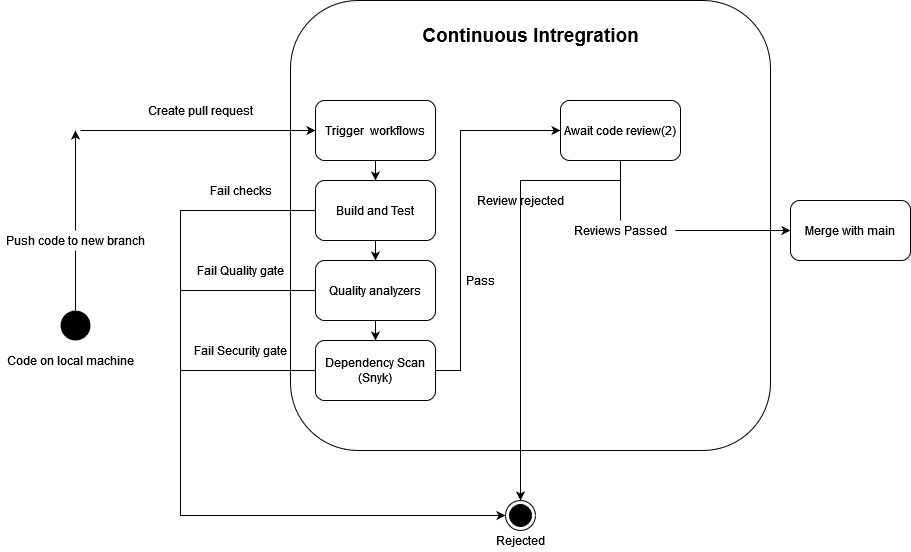
\includegraphics[scale=0.50]{images/ci_cd_diagrams/DevopsDiagrams-StateMachine CI.drawio(4).png}
    \caption{CI Pipeline State Machine Diagram}
    \label{fig:CIStateMachine}
\end{figure}
As shown in Figure \ref{fig:CIStateMachine}, if any of these fail, the CI pipeline will direct to a rejected state. Once all workflows are passed, the pull request awaits review until at least two developers have approved it. Afterwards, changes can be merged into the main branch.

\subsubsection{CD - Continuous Delivery/Deployment}
\label{subsubsec:cd}

Our pipeline introduces a mix of Continuous Delivery and Continuous Deployment(Illustrated in Figure \ref{fig:CDStateMachine}). Deployment is done by the deployment workflow(cluster-deploy.yml).
The workflow is triggered every time a release is created. It also supports manual dispatch for hot fixing errors, and the weekly release workflow runs every Sunday evening, triggering the deployment pipeline. The deployment workflow is comprised of 4 jobs.
\begin{enumerate}
    \item \textbf{.Net Build and Test} - This job is described in \ref{subsubsec:ci}.
    \item \textbf{Build and Push containers} - Builds, tags, and pushes containers to docker hub. We can then pull all necessary containers from docker hub.
    \item \textbf{Snyk Dependency scan} - Security gate. If a risk exceeds the gate, deployment will stop immediately and move to the canceled state. See Figure \ref{fig:CDStateMachine}
    \item \textbf{Dispatch} - Dispatches the apply workflow in the Operations repository.
\end{enumerate}

\begin{figure}[H]
    \centering
    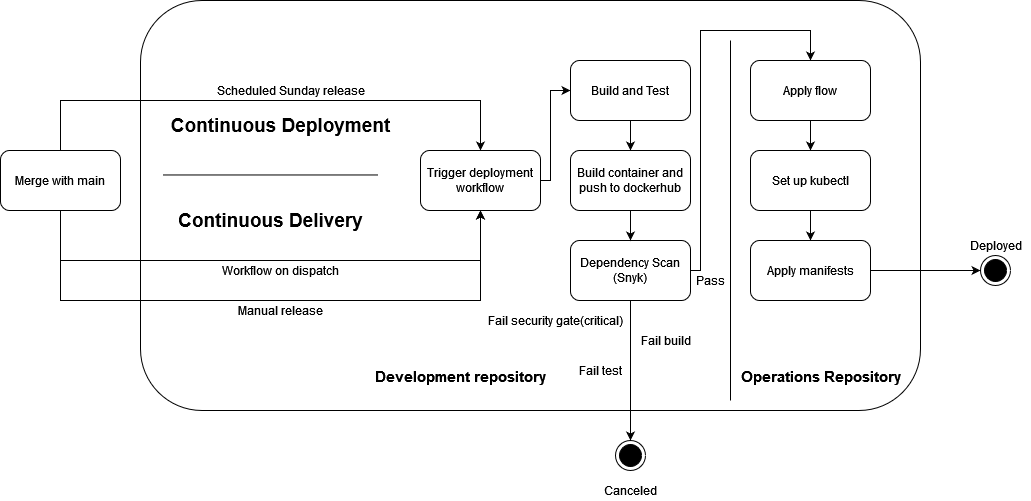
\includegraphics[scale=0.44]{images/ci_cd_diagrams/DevopsDiagrams-StateMachineCd.drawio.png}
    \caption{CD Pipeline State Machine Diagram}
    \label{fig:CDStateMachine}
\end{figure}

When the \textit{apply} workflow has been dispatched, the runner will set up kubectl using a Digital ocean token, with the cluster name saved as secrets in the repository. The apply shell script is executed, which "applies" all the configuration manifests, thus deploying the changes.

\subsection{Version Control}
\label{subsec:vs}
% Organization of your repositor(ies).
% That is, either the structure of of mono-repository or organization of artifacts across repositories.
% In essence, it has to be be clear what is stored where and why
\subsubsection{Organization of Repositories}
There is a total of 3 repositories Dev Repository (see \ref{app:devRepo}) and 2 submodules: Ops Repository (see \ref{app:opsRepo}) and \href{https://github.com/Akongstad/DevOps-Report}{Report Repository}.
\subsubsection{Branching Strategy}

% - Applied branching strategy.
% For example, how did you use issues, Kanban boards, etc. to organize open tasks

Our organization uses a Trunk Based Development branching model. We have two centralized branches, which were continuously debugged, tested, and in a working state. Features, patches, and bug fixes are always developed on dedicated temporary branches, which are deleted after being merged into their relative centralized branch.\\

\textbf{Dev Repository @ main} (see \ref{app:devRepo})\\\\
The \textbf{main} branch lives on GitHub and is the alpha of our centralized workflow. While we develop features and patches on temporary branches, everything worthwhile is eventually merged into main. \\

Primary applications of the main branch are:
\begin{enumerate}
    \item Store working source code
    \item Make releases
    \item Run workflows
    \item Build and push docker images\\
\end{enumerate}

\textbf{Ops Repository @ master} \ref{app:opsRepo}\\\\
The master branch of the Ops repository contains infrastructure as code for creating and configuring a Kubernetes cluster, manifest files used to deploy our service to the cluster, and shell scripts for automating these steps.

\subsection{Development process and tools}
\label{subsec:process&tools}
% - Applied development process and tools supporting it
GitHub issues track progress of tasks. Upon creation, issues are tagged and organized into GitHub Projects. By using a combination of issues, projects, and enforcement of code reviews, we promote transparency between developers, thus making sure to share progress and knowledge between developers.

\subsection{Monitoring And Logs}
\label{subsec:monitoring}
Monitoring is implemented by the Prometheus microservice, which scrapes a list of endpoints for PromQL metrics every 5s.
The PromQL data is formatted and displayed by the Grafana microservice which is publicly accessible.
% How do you monitor your systems and what precisely do you monitor?
% What do you log in your systems and how do you aggregate logs?
\subsubsection{Software Quality Definitions}
\label{subsubsec:software_quality_definitions}
The following definitions provide a clearer image of desirable metrics for monitoring \mini and analyzing logs.
\begin{table}[H]
    \centering
    \begin{tabular}{|c|p{6cm}|}\hline
        Robustness & The predictability of our software's response to unexpected input  \\\hline
        Functionality & The predictability of our software's response to expected input \\\hline
        Performance & The efficiency of resource usage \\ \hline
    \end{tabular}
    \caption{Definitions of Software Quality}
    \label{tab:software_quality}
\end{table}

\subsubsection{Metrics}
From the definitions of software quality in table \ref{tab:software_quality} the metrics in table \ref{tab:metrics} were derived.

\begin{table}[H]
    \centering
    \begin{tabular}{|c|c|} \hline
        Robustness & Server error response count \\
        & Client error response count \\ \hline
        Functionality & API mean response time  \\ 
        & API endpoint call count \\
        & API endpoint error count  \\ \hline
        Performance & Host memory usage \\
        & Host CPU load \\ \hline
    \end{tabular}
    \caption{Metrics derived from definitions of software quality}
    \label{tab:metrics}
\end{table}

\subsubsection{Logging}
Logging was temporarily implemented with the ELK stack but proved to be unsustainable with the resources at hand.
Logs are generally categorized by levels. 
The definitions of the levels vary from system to system but their range is consistently between "Debug" and "Error".
The ELK stack was configured to scrape logs from STDOUT and STDERR from frontend and backend microservices which proved sufficient.

\subsection{Security}
\label{subsec:security}
To discover, define, and asses vulnerabilities of our system, we have conducted a security assessment and a pen-test. This section includes only selected results(see Appendix\ref{app:secAss} for more).

Using the OWASP Top 10\cite{owasp} we identified possible insecurities in our system. We constructed risk scenarios and analyzed their likelihood and impact. 
The analysis yielded "\textit{Outdated Components}" as a top concern. As security breaches are discovered half a year later on average, the way to combat security threats is proactivity\cite{securitylecture}. To decrease chance of having outdated components in production, we added Dependabot to our GitHub repository. Dependabot creates pull requests automatically suggesting updating outdated components. Snyk, which was mentioned in \ref{subsubsec:code_quality} scans the repository for vulnerabilities sand sensitive data leaks. Handling of secrets to prevent leaks is described in \ref{subsubsec:secrets}.
We conducted an automated penetration test to:
\begin{enumerate}
    \item Detect vulnerabilities
    \item Test the system under stress
\end{enumerate}
Using the logging system, we noticed the server received requests from all around the world, e.g. Nevada. In conclusion, except for acting as a DOS attack on our own system, eventually crashing the ELK stack. Pen testing did not yield any system vulnerabilities.

\subsubsection{Secret Handling}
\label{subsubsec:secrets}
Securing sensitive data while allowing access to multiple parties is challenging. We use GitHub secrets for securing tokens and keys that are accessed and injected into our CI/CD pipeline. Alternatively, we have a local folder containing the database connection string, database-password, and jwt token key, all shared through discord. Security could be improved by splitting the key into multiple parts and sharing them separately. However, we deemed this excessive.
\clearpage
\subsection{Scaling And Load balancing}
\label{subsec:scaling}
% Applied strategy for scaling and load balancing.
%Include reflection over why scaling and load balancing benefit us, why kubernetes might have been overkill for the project, but which pros and cons we considered when deciding.

\subsubsection{Single server setup}
\label{subsubsec:scalingProd}
The original single server setup is located on \textbf{Dev Repository @ production} (see \ref{app:devRepo}), and can be seen in Figure \ref{fig:legacyDeploy}.
Although now deprecated, the production branch had our production server and was our main branch's lean and automated counterpart. It was developed such that our multi-container application could be rebuilt and updated on the production server to include updated Docker images and changes in configuration files with a single command, minimizing downtime without using load-balancers.\\
Only vertical scaling using the digital ocean API was possible. It will become exceedingly more expensive as more virtual CPU cores, RAM, and disk space is added, eventually reaching an upper limit. The single monolithic VM will forever be a single point of failure, and upgrading the VM will require the server shut down.
\begin {figure}[H]
    \centering
    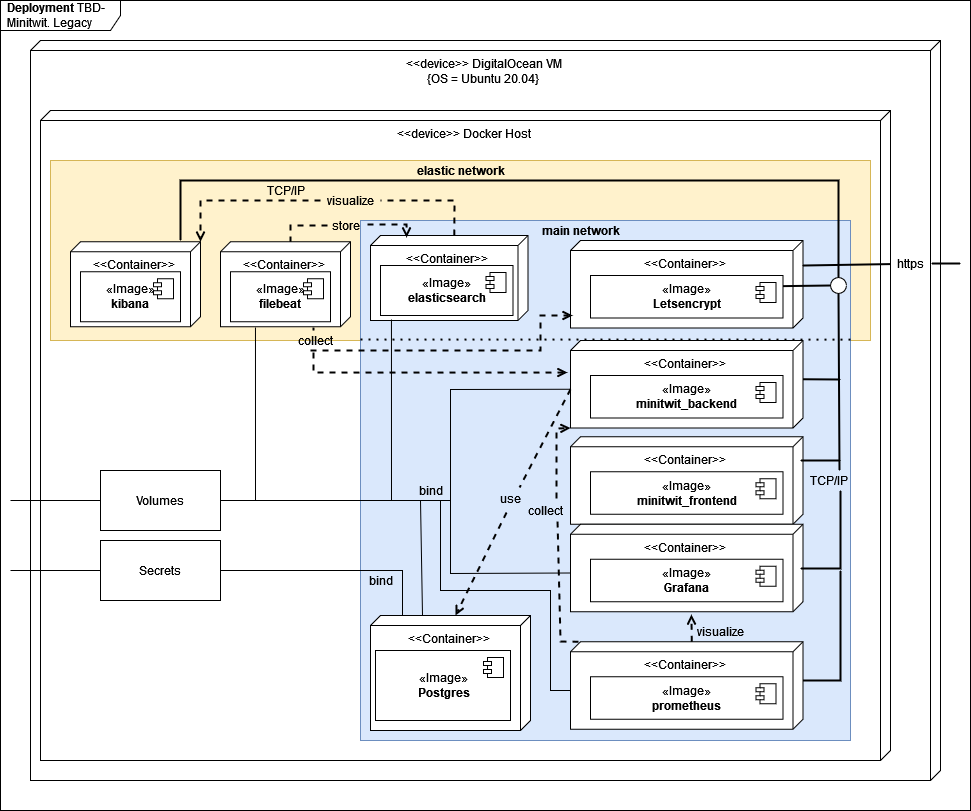
\includegraphics[scale=0.47]{images/deployment_diagrams/DevopsDiagrams-Legacy deploy mini.drawio.png}
    \caption{\mini single server deployment diagram}
    \label{fig:legacyDeploy}
\end{figure}

\subsubsection{Scaling the application}
\label{subsubsec:scalingApp}
Eliminating the server as a single point of failure while allowing for rolling updates out without shutting down the application could be accomplished by introducing a setup with a primary server and backup server while swapping around IPs, but that would not allow for horizontal scaling.\\
Options that, out of the box, come with horizontal scaling, load balancing, and rolling updates while eliminating the single point of failure include container orchestration tools like Docker Swarm and Kubernetes.\\ 
We have chosen to migrate our application to a Kubernetes cluster. One can argue that the additional complexity and setup required for deploying a Kubernetes cluster is unnecessary since Docker Swarm fulfills our requirements, thus conflicting with the simplicity principle: "\textit{Simplicity--the art of maximizing the amount of work not done--is essential}"\cite{beck2001agile}. 
One reason for this choice is that documentation on the setup and management of a Kubernetes cluster was significantly more extensive, although the increased complexity might cause that. Secondly, we wished to gain experience using Kubernetes for container orchestration. That said, automated scaling\footnote{\url{https://kubernetes.io/}} does save time for developers, even if monitoring service load and manually scaling a swarm when required is a possible solution. In conclusion, by migrating to a Kubernetes cluster, we support horizontal scaling, load balancing, and rolling updates. However, we must admit that even though the database was flushed and deployed to the cluster, we do not have a replicated database because of consistency concerns and can therefore not claim to have eliminated all single points of failure.
